\section{ASP.NET MVC architektúra}

\indent Az államvizsga-dolgozatom célja bemutatni egy webalapú alkalmazás fejlesztési folyamatát és technológiai hátterét, amely egy buszvállalat működését támogatja. A fejlesztés során az ASP.NET MVC keretrendszerre építek, amely jól strukturált megközelítést kínál a webes alkalmazások építéséhez, miközben lehetővé teszi az üzleti logika, a megjelenítés és az adatkezelés hatékony szétválasztását.

A dolgozat első fejezete a .NET platform által kínált lehetőségekre és az MVC (Model-View-Controller) architektúra alapelveire összpontosít. Részletesen ismertetjük a modell, a nézet és a vezérlő szerepét, valamint ezek együttműködését a rendszer működésében. Külön figyelmet fordítunk az útvonalkezelés és az adatátadás mechanizmusaira is, amelyek az ASP.NET MVC egyik kulcsfontosságú komponensét jelentik.

A következő alfejezetekben bemutatásra kerülnek azok a technológiák, amelyek kiegészítik és támogatják az alkalmazás működését. Az Entity Framework révén az adatbázis-kezelés objektumorientált módon valósul meg, míg a Razor nézetmotor a dinamikus tartalmak hatékony megjelenítését teszi lehetővé. A kliensoldali működéshez elengedhetetlen JavaScript mellett a Leaflet könyvtár térképes vizualizációt biztosít, amely különösen hasznos a szállítási útvonalak megjelenítéséhez. A rendszer részeként implementált e-mail értesítések SMTP protokollon keresztül működnek, míg a QR-kód generálás lehetőséget nyújt például jegyek, csomagazonosítók vagy beléptetési információk digitális tárolására és gyors elérésére.

\begin{figure}[H]
    \centering
    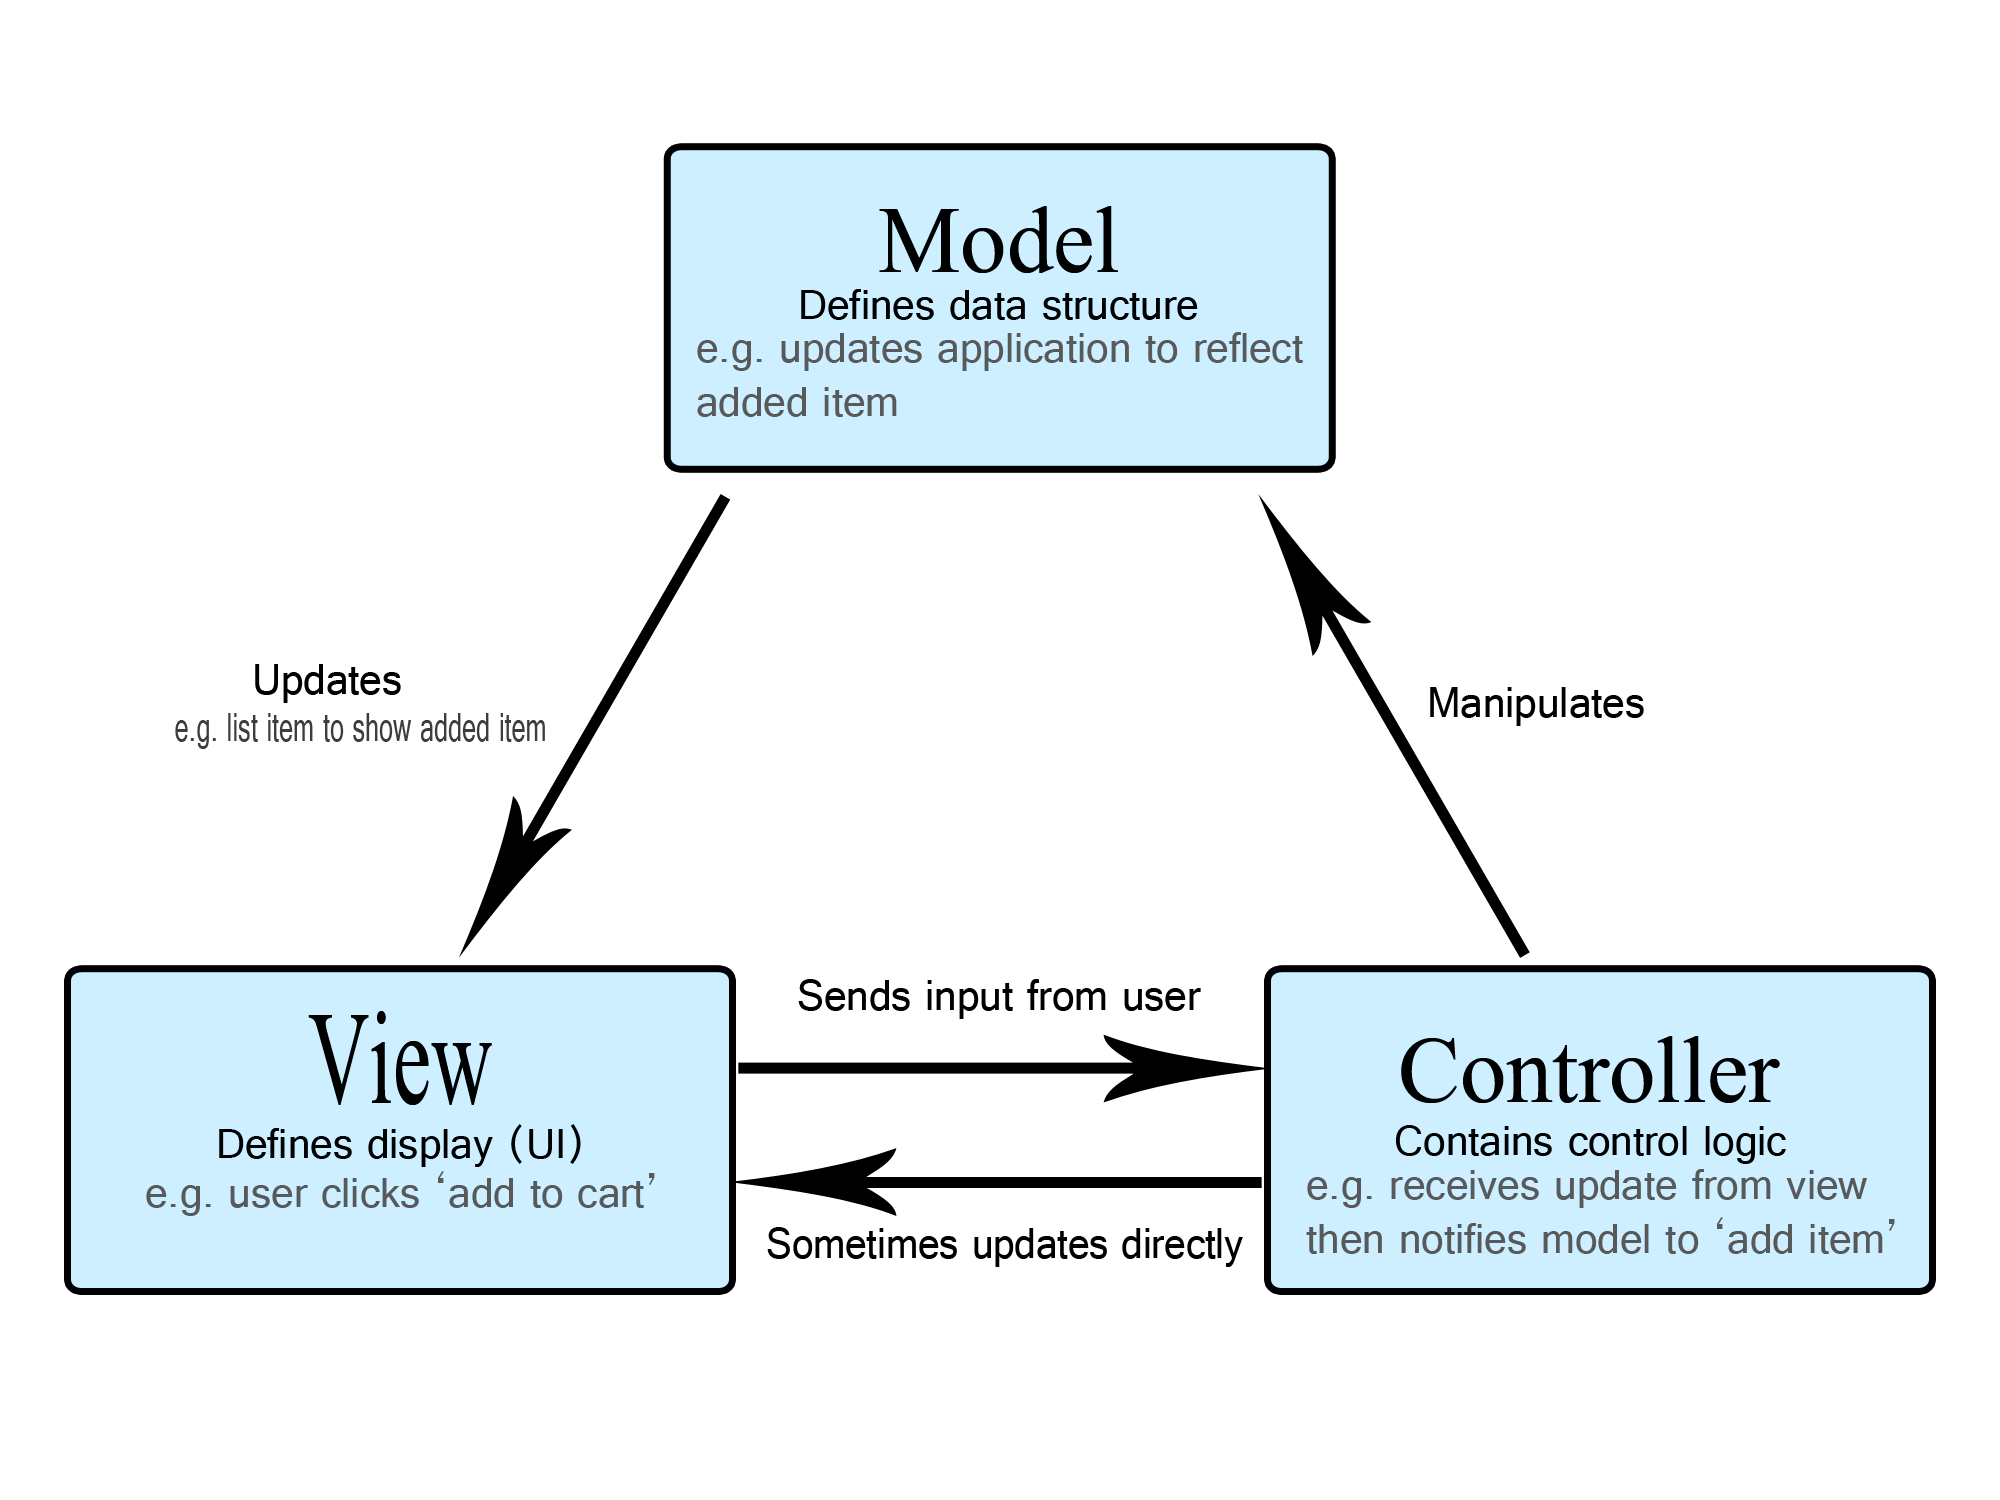
\includegraphics[width=1\textwidth]{Szakdolgozat/Mellekletek/model-view-controller-light-blue.png}
    \caption{Az MVC (Model–View–Controller) architektúra felépítése. Az ábrán jól látható, hogyan különül el az adatkezelés (Model), a felhasználói felület (View) és az üzleti logikát kezelő vezérlő (Controller). Az egyes rétegek közötti kommunikáció segíti az alkalmazás moduláris, karbantartható és tesztelhető kialakítását. (Forrás: MVC Architektúra – MDN Web Docs)}
    \label{fig:er-diagram}
\end{figure}


\subsection{A .NET platform és az MVC minta}

\indent A .NET egy többnyelvű, keresztplatformos fejlesztési környezet, amelyet a Microsoft hozott létre, és amely lehetőséget nyújt különböző típusú alkalmazások – például asztali, webes és mobil – fejlesztésére. A platform célja, hogy egységes, megbízható és jól skálázható környezetet biztosítson a fejlesztők számára. Ezen belül az ASP.NET a webalkalmazások készítésére szolgáló keretrendszer, amely támogatja az MVC (Model–View–Controller) mintát.

Az MVC architektúra egyik legfontosabb előnye az alkalmazás logikájának, adatainak és felhasználói felületének elkülönítése. Ez nemcsak a kód tisztaságát és átláthatóságát javítja, hanem lehetővé teszi a különböző fejlesztői szerepkörök (pl. backend, frontend) hatékony együttműködését, valamint a rendszer egyszerűbb tesztelhetőségét és karbantarthatóságát.

\subsection{A .NET platform és az MVC minta}

\indent A projekt megvalósításához az ASP.NET Core technológiát választottam, amely a Microsoft által fejlesztett modern, nyílt forráskódú és platformfüggetlen fejlesztői keretrendszer része. A .NET környezet lehetővé teszi különféle típusú alkalmazások – többek között webes, asztali és mobil – egységes és hatékony fejlesztését. Az ASP.NET Core kifejezetten a webes alkalmazások készítésére lett optimalizálva, és kiválóan támogatja a korszerű biztonsági és teljesítménybeli elvárásokat. 

A .NET választása mellett szólt annak kiforrottsága, az általa nyújtott bőséges dokumentáció és eszköztámogatás, valamint az a tény, hogy Visual Studio környezetben fejlesztve a hibakeresés és a tesztelés is jól integráltan megoldható. Alternatívaként szóba jöhetett volna például a Java Spring Boot keretrendszer vagy a Node.js + Express kombináció is, azonban ezek konfigurációs szempontból komplexebbek lehetnek , és az Identity típusú autentikációs és jogosultságkezelési rendszerek bevezetése is jelentősebb többletmunkát igényel.

A projekt architektúráját az MVC (Model–View–Controller) mintára építettem. Ez a tervezési minta a szoftverfejlesztésben széles körben alkalmazott struktúra, amely szétválasztja az adatkezelésért felelős réteget (Model), a megjelenítést (View), valamint a vezérlő logikát (Controller). Ennek az elkülönítésnek köszönhetően az alkalmazás fejlesztése átláthatóbbá válik, a komponensek tesztelése könnyebben megvalósítható, és a hosszú távú karbantarthatóság is biztosított.

Webes alkalmazást szerettem volna fejleszteni, ebből kiindúlva itt mutatkozik meg az MVC minta előnye: az adatok és a nézetek logikai szétválasztása segít elkerülni a kóduplikációt, és támogatja a front- és backend fejlesztés párhuzamos végzését. A moduláris struktúra továbbá lehetőséget ad az egyes komponensek újrafelhasználására is, ami a jövőbeni bővítéseket és új funkciók integrálását jelentősen megkönnyíti, ezért is esett erre a választásom. Egy másik fontos érv az MVC arhitekúra választása mellett, hogy számomra ez egy nagyon jól átláthatóv valamint kivitelezhető arhitekúra.

\subsubsection{ASP.NET MVC alapelvei}

\indent Az ASP.NET MVC keretrendszer három jól elkülöníthető rétegre bontja az alkalmazás struktúráját. A Model réteg felelős az üzleti logika és az adatok kezeléséért, a View a felhasználó számára megjelenített tartalmat írja le, míg a Controller a két réteg közötti kommunikációért és az események kezeléséért felel. Ez az elkülönítés elősegíti az egységek külön történő fejlesztését és tesztelését.

Az ASP.NET MVC a REST architektúra alapelveit követi, és szorosan épít az URL-alapú útvonalkezelésre (routing), amely meghatározza, hogy egy adott kérés melyik vezérlőhöz és metódushoz kerüljön. (Forrás: MVC Architektúra – MDN Web Docs)

\subsubsection{A Controller, View és Model szerepe}

\indent A Controller felelős a beérkező HTTP-kérések kezeléséért, az adatok lekérdezéséért vagy módosításáért, és végül az adatok továbbításáért a View felé. A Model tartalmazza az alkalmazás által kezelt adatokat és azok viselkedését, gyakran adatbázissal kapcsolatban álló entitások és azok logikája formájában. A View Razor szintaxisban írt .cshtml fájlokat jelent, amelyek HTML-ben jelenítik meg a Modelből származó adatokat, ezzel biztosítva a dinamikus tartalom megjelenítését.(Forrás: MVC Architektúra – MDN Web Docs)

\subsubsection{Routing és adatátadás}

\indent Az útvonalkezelés (routing) kulcsszerepet játszik az ASP.NET MVC működésében. Az URL-ek mintákat követnek, amelyek alapján a rendszer eldönti, hogy melyik Controller és azon belül melyik Action metódus hajtódjon végre. Az adatok átadása történhet route paramétereken, query stringen vagy formokon keresztül, míg az adatok feldolgozását és továbbítását a Controller végzi, amely továbbküldi azokat a View vagy más üzleti logikai rétegek számára. (Forrás: MVC Architektúra – MDN Web Docs)


\subsection{Kapcsolódó technológiák}

\subsubsection{Entity Framework és az adatkezelés integrációja}

\indent Az Entity Framework (EF) a .NET keretrendszer objektum-relációs leképezést (ORM) alkalmazó technológiája, amely lehetővé teszi, hogy az adatbázis-műveleteket magas szintű, típusosan definiált C\# osztályokon keresztül végezzük el. Az EF célja, hogy a relációs adatbázisokkal való munka során elrejtse a nyers SQL lekérdezések szükségességét, ezáltal elősegítve a biztonságosabb és karbantarthatóbb adatkezelést.

Az EF támogatja a különböző adatmodellezési megközelítéseket, köztük a Code First és Database First stratégiákat. A Code First megközelítés lehetővé teszi, hogy a fejlesztők először az osztálystruktúrát hozzák létre a C\# nyelv eszközeivel, majd az EF automatikusan létrehozza és karbantartja a hozzá tartozó adatbázis-sémát. Ezzel szemben a Database First modell olyan helyzetekben előnyös, ahol már létező adatbázis-struktúrához kell alkalmazkodni.

Az alkalmazás adatbázis-kommunikációja általában Microsoft SQL Serverrel történik, amely a .NET ökoszisztémán belül natívan támogatott. Az EF SQL Serverrel való összekapcsolását a DbContext konfigurálásán keresztül végezzük, ahol a kapcsolat elérési adatai (connection string) egy konfigurációs fájlban vagy programkódban definiálhatók. A kapcsolat biztonságos kezeléséhez jellemzően Windows hitelesítést vagy SQL Server hitelesítést használunk, opcionálisan SSL titkosítással.

A modern ASP.NET alapú alkalmazásokban az EF szorosan együttműködik az ASP.NET Identity keretrendszerrel, amely a felhasználókezelési és hitelesítési feladatokat látja el. Az Identity rendszer szintén az EF-en keresztül valósítja meg a felhasználói adatok (pl. regisztrációs információk, jelszavak hash-elve, jogosultságok, szerepkörök) tartós tárolását és kezelését. A felhasználói entitások a többi modellosztályhoz hasonlóan entitásként jelennek meg az adatbázisban, így az EF által biztosított LINQ-lekérdezések és migrációs eszközök teljes mértékben alkalmazhatók rájuk is.

Ez az integrált megközelítés lehetővé teszi, hogy az alkalmazás egységes módon kezelje mind az üzleti, mind az autentikációs adatokat, miközben biztosítja az adatbázis-struktúra automatikus frissítését és bővítését a fejlesztés során.(Forrás: Entity Framework Core – Microsoft Docs)

\subsubsection{Razor nézetek}

\indent A felhasználói felület dinamikus generálásához a Razor nézetmotor alkalmazása mellett döntöttem, amely az ASP.NET Core keretrendszerbe szorosan integrált megoldás. A Razor lehetővé teszi a HTML markup és a C\# nyelvi elemek egységes szintaxisban történő használatát, így a nézetek logikusan felépíthetők és karbantarthatók. A Razor-fájlok \texttt{.cshtml} kiterjesztéssel rendelkeznek, és szerves részét képezik az alkalmazás prezentációs rétegének.

A Razor szintaxis kiválasztása elsődlegesen a következő gyakorlati szempontok alapján történt: az egyszerűség, a tisztaság és a beépített funkcionalitás. A Razor nézetek képesek közvetlenül hozzáférni a modell objektumaihoz, és a C\# nyelv erejét felhasználva hatékonyan képesek kiszolgálni a dinamikus tartalmak megjelenítését. A kód és a megjelenítés szétválasztása továbbra is biztosított, mivel az üzleti logika nem kerül közvetlenül a nézetfájlokba, így az architektúra továbbra is tiszta és jól strukturált marad.

Alternatívaként lehetőség lett volna JavaScript-alapú frontend könyvtárak – például React, Angular vagy Vue – alkalmazására is, azonban ezek esetében jelentős többletkonfigurációra és különálló frontend-backend struktúra kialakítására lett volna szükség. Bár ezek a megoldások kiválóan alkalmasak nagy felhasználói interakciókat igénylő, erősen kliensoldali alkalmazások fejlesztésére, a jelen projekt célkitűzéseihez egy szerveroldali, egyszerűen karbantartható megoldás sokkal jobban illeszkedett.


\indent A megjelenítés esztétikai és felhasználói élménybeli szempontból történő javítása érdekében a Razor nézetekben gyakran alkalmazzák a Bootstrap keretrendszert, amely előre definiált, reszponzív stílusokat és elrendezéseket kínál. Emellett elterjedt a Bootstrap Icons (BI) használata is, amely vektor alapú ikonokat biztosít a vizuális elemek kiegészítésére és gazdagítására. Ezen eszközök integrálása nemcsak a fejlesztési folyamatot gyorsítja fel, hanem hozzájárul a konzisztens és professzionális megjelenés kialakításához is.(Forrás: Razor View Engine (ASP.NET Core 8.0) – Microsoft Docs)

\subsubsection{Leaflet}

\indent A térképes megjelenítéshez a Leaflet könyvtárat választottam, amely egy nyílt forráskódú, könnyen használható és rendkívül testreszabható JavaScript-alapú megoldás. Kifejezetten hatékony interaktív térképek beágyazására, amelyek lehetővé teszik megállók, útvonalak és helyadatok vizuális reprezentálását. Mindez különösen fontos volt egy közlekedési alkalmazás esetében, ahol az információk térbeli megjelenítése lényeges felhasználói igény.

A Leaflet előnye a kis méret és a teljesítmény mellett a könnyű integrálhatóság ASP.NET alkalmazásokba. A könyvtár támogatja az OpenStreetMap-alapú térképek használatát, így licencdíjmentes és korlátozás nélkül használható akár prototípus-fejlesztéshez, akár éles rendszerekhez. Számos bővítmény áll rendelkezésre, például marker clustering, útvonalrajzolás, amelyek mind a projekt céljait szolgálták.

Alternatív megoldásként szóba jöhetett volna a Google Maps API vagy a Mapbox használata is. Ezek a szolgáltatások bár rendkívül fejlettek és látványos térképes megoldásokat kínálnak, jelentős hátrányuk, hogy hosszabb távon anyagi terhet jelenthetnek a kvótákon alapuló árazási modell miatt. 

A Leaflet tehát nemcsak technikailag bizonyult megfelelőnek, hanem stratégiai döntésként is helytállt: biztosította a térképes funkcionalitást egy egyszerűen használható, megbízható és ingyenes megoldás keretében. Az alkalmazás vizuális élményét jelentősen növelte, miközben minimálisra csökkentette az erőforrásigényt, és könnyen testreszabható maradt a későbbi fejlesztésekhez.(Forrás: Leaflet – JavaScript térképkönyvtár)

\subsubsection{E-mailküldés SMTP protokollal}


\indent A felhasználói visszaigazolások, regisztrációk és rendszerüzenetek továbbításához elengedhetetlenné vált az e-mailes kommunikáció beépítése a rendszerbe. A megvalósításhoz az SMTP (Simple Mail Transfer Protocol) protokollt választottam, amely szabványos, platformfüggetlen megoldást nyújt a levelek kézbesítésére. Az implementációhoz a .NET keretrendszer \texttt{System.Net.Mail} bővítményt használtam, amely közvetlen lehetőséget biztosít levelek küldésére különféle hitelesítési és biztonsági beállítások mellett.

A választás fő indoka a közvetlen integráció és egyszerűség: mivel ez a megoldás nem igényel külső csomagokat vagy szolgáltatásokat, könnyen testre szabható, jól kontrollálható és független bármilyen e-mail szolgáltatótól. A konfiguráció során lehetőség nyílt az SSL/TLS biztonsági réteg használatára, az SMTP host, port és felhasználói adatok megadására, így teljes mértékben testreszabhatóvá vált az üzenetküldés folyamata. (Forrás: SmtpClient Class – Microsoft Docs)

\subsubsection{QR-kód generálás}

\indent A QR-kódok (Quick Response Code) egyre elterjedtebb eszközei a digitális azonosításnak és információátadásnak, különösen a közlekedési, jegyértékesítési és beléptetési rendszerek esetében. Az alkalmazásban ezek a kódok a digitális jegyek részét képezik, lehetővé téve a gyors és egyszerű beazonosítást vizuális beolvasással. A megoldás célja az volt, hogy a felhasználók egyedi, könnyen kezelhető és hordozható formában juthassanak hozzá jegyeikhez.

A QR-kód generálásához a \texttt{QRCoder} nevű .NET kompatibilis nyílt forráskódú könyvtárat használtam, amely egyszerű API-t biztosít bitmap vagy SVG formátumú QR-kódok létrehozásához. A választás mellett szólt, hogy ez a könyvtár könnyedén integrálható az ASP.NET MVC projektekbe, nem igényel különösebb konfigurációt, és elegendő rugalmasságot nyújt ahhoz, hogy különféle típusú adatokat (pl. URL, egyedi azonosító) kódoljunk benne.

A rendszerben minden jegyfoglalás után automatikusan létrejön egy egyedi QR-kód, amely tartalmazza az adott jegyhez kapcsolódó azonosítót. Ez a megoldás nemcsak a felhasználói élményt növeli – hiszen nem szükséges kinyomtatott jegyet magukkal vinniük –, hanem előkészíti az esetleges jövőbeli bővítéseket is, például a mobilos beolvasáson alapuló beléptetési rendszer irányába.(Forrás: Creating QR Code in ASP.NET Core – C\# Corner)
